\documentclass[11pt,a4paper]{report}
\usepackage{graphicx}
\begin{document}
\title{Cloud Computing}
\author{Cloud Computing Research Paper for CS308 \\Supervisor: Dr/Abd El-Aziz El Damaran \\
\\Mahmoud Aref 110747\\Ramy Mohamed\\Mahmoud Adel\\Ahmed Sayed 130806}
\date{May 2016}
\maketitle
\chapter{Introduction to Cloud Storage system}

\subsection{Cloud Computing}

Cloud computing has emerged as a promising technique that greatly changes the modern IT industry. The National Institute of Standards and Technology (NIST) defined the cloud computing as follows  Cloud computing is a model for enabling convenient, on-demand network access to a shared pool of configurable and reliable computing resources(e.g., networks, servers, storage, applications, services) that can be rapidly provisioned and released with minimal consumer management effort or service provider interaction.This cloud model is composed of Five essential characteristics,three service models, and four deployment models.

\subparagraph*{The Five essential characteristics are defined as:}
\begin{itemize} 
\item on-demand self-service
\item Ubiquitous network access
\item Resource pooling
\item Rapid elasticity or expansion 
\item Measured service 
\end{itemize}
\begin{figure}
\centering
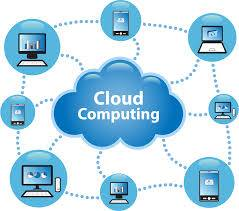
\includegraphics[width=0.3\textwidth]{4.jpg}
\caption{\label{Cloud Computing}}
\end{figure}


\subparagraph*{The service models are defined as :}
\subparagraph*{Cloud Software as a Service (SaaS)} 
 Use providers applications over a network. 

\subparagraph*{The benefits of SaaS (Software as a system) :}
\begin{itemize}
\item You can sign up and rapidly start using innovative business apps
\item Apps and data are accessible from any connected computer
\item No data is lost if your computer breaks, as data is in the cloud
\item The service is able to dynamically scale to usage needs
\end{itemize}
\subparagraph*{Cloud Platform as a Service (PaaS)}
Deploy customer-created applications to a cloud.
\subparagraph{The benefits of PaaS (Platform as a service)}
\begin{itemize}
\item Develop applications and get to market faster
\item Deploy new web applications to the cloud in minutes
\item Reduce complexity with middleware as a service
\end{itemize}
\subparagraph*{Cloud Infrastructure as a Service (laaS)}
Rent processing,storage,network capacity, and other fundamental computing resources.
\subparagraph*{The benefits of IaaS (Infrastructure as a system)}
\begin{itemize}
\item No need to invest in your own hardware
\item Infrastructure scales on demand to support dynamic workloads
\item Flexible, innovative services available on demand
\end{itemize}
\subparagraph*{The deployment models,summarized in the NIST definition as : }
\subparagraph*{Public cloud(Sold to the public, mega-scale infrastructure)} 
Public clouds are owned and operated by companies that offer rapid access over a public network to affordable computing resources. With public cloud services, users don’t need to purchase hardware, software, or supporting infrastructure, which is owned and managed by providers.
\begin{figure}
\centering
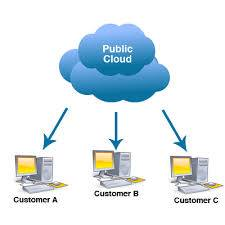
\includegraphics[width=0.3\textwidth]{1.jpg}
\caption{\label{Public Cloud}  }
\end{figure}
\subparagraph*{Key aspects of public cloud}
\begin{itemize}
\item Innovative SaaS business apps for applications ranging from customer resource management (CRM) to transaction management and data analytics
\item Flexible, scalable IaaS for storage and compute services on a moment`s notice.

\item Powerful PaaS for cloud-based application 	development and deployment environments
\end{itemize}
\subparagraph*{Private cloud}
A private cloud is infrastructure operated solely for a single organization, whether managed internally or by a third party, and hosted either internally or externally. Private clouds can take advantage of cloud’s efficiencies, while providing more control of resources and steering clear of multi-tenancy.
\begin{figure}
\centering
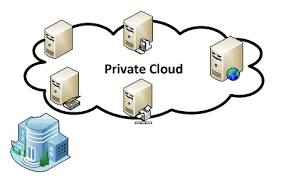
\includegraphics[width=0.3\textwidth]{4.png}
\caption{\label{Private Cloud}}
\end{figure}
\subparagraph*{Key aspects of private cloud}
\begin{itemize}
\item A self-service interface controls services, allowing IT staff to quickly provision, allocate, and deliver on-demand IT resources
\item Highly automated management of resource pools for everything from compute capability to storage, analytics, and middleware
\item Sophisticated security and governance designed for a company`s specific requirements.
\end{itemize}
\subparagraph*{Hybrid cloud (Composition of two or more clouds)}
A hybrid cloud uses a private cloud foundation combined with the strategic integration and use of public cloud services. The reality is a private cloud can’t exist in isolation from the rest of a company’s IT resources and the public cloud. Most companies with private clouds will evolve to manage workloads across data centers, private clouds, and public clouds—thereby creating hybrid clouds.
\begin{figure}
\centering
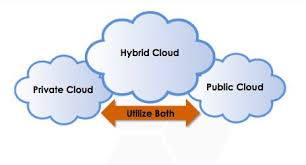
\includegraphics[width=0.3\textwidth]{2.jpg}
\caption{\label{Hybird Cloud}}
\end{figure}
\subparagraph*{Key aspects of hybrid cloud}
\begin{itemize}
\item Allows companies to keep the critical 	applications and sensitive data in a traditional 	data center environment or private cloud.
\item Enables taking advantage of public cloud 	resources like SaaS, for the latest applications, 	and IaaS, for elastic virtual resources
\item Facilitates portability of data, apps and services 	and more choices for deployment models
\end{itemize}
\subparagraph{Community cloud}
 Shared infrastructure for specific community       
\subsection{Cloud Storage as a Service}
Cloud storage is an important service of cloud computing,which allows data owners (owners) to host data from their local computing systems to the cloud, Cloud storage is a model of networked online storage where data is stored in virtualized pools of storage which are generally hosted by third parties(e.g.,the storage service providers). The service providers operate large data centers, and data owners buy or lease storage capacity from them in a pay-as-you-go business model.
\\The service providers, in the background, virtualize the resources according to the requirements of the customer and expose them as storage pools, which the customers can themselves use to store files or data objects. Physically, the resource may span across multiple servers.
 \paragraph{Cloud Storage Benefits}
 test
 \begin{itemize}
\item Usability:All cloud storage services reviewed in this topic have desktop folders for Mac’s and PC’s. This allows users to drag and drop files between the cloud storage and their local storage.
\item Bandwidth:You can avoid emailing files to individuals and instead send a web link to recipients through your email.
\item Accessibility:Stored files can be accessed from anywhere via Internet connection.
\item Disaster Recovery It is highly recommended that businesses have an emergency backup plan ready in the case of an emergency. Cloud storage can be used as a back‐up plan by businesses by providing a second copy of important files. These files are stored at a remote location and can be accessed through an internet connection.
\item Cost Savings:Businesses and organizations can often reduce annual operating costs by using cloud storage; cloud storage costs about 3 cents per gigabyte to store data internally. Users can see additional cost savings because it does not require internal power to store information remotely.
\end{itemize}
\paragraph{Disadvantages of Cloud Storage}
\begin{itemize}
\item  Usability:Be careful when using drag/drop to move a document into the cloud storage folder. This will permanently move your document from its original folder to the cloud storage location. Do a copy and paste instead of drag/drop if you want to retain the document’s original location in addition to moving a copy onto the cloud storage folder.
\item Bandwidth:Several cloud storage services have a specific bandwidth allowance. If an organization surpasses the given allowance, the additional charges could be significant. However, some providers allow unlimited bandwidth. This is a factor that companies should consider when looking at a cloud storage provider.
\item Accessibility:If you have no internet connection, you have no access to your data.
\item Data Security:There are concerns with the safety and privacy of important data stored remotely. The possibility of private data commingling with other organizations makes some businesses uneasy. If you want to know more about those issues that govern data security and privacy, here is aninteresting article on the recent privacy debates.
\item Software:If you want to be able to manipulate your files locally through multiple devices, you’ll need to download the service on all devices.
\end{itemize}

\chapter{ARCHITECTURE OF CLOUD COMPUTING}
\section{introduction}
In this section, we present a top-level architecture of cloud computing that depicts various cloud service delivery models.Cloud computing enhances collaboration, agility, scale, availability and provides the potential for cost reduction through optimized and efficient computing. More specifically, cloud describes the use of a collection of distributed services, applications, information and infrastructure comprised of pools of compute, network, information and storage resources\\These
components can be rapidly orchestrated, provisioned, implemented and decommissioned using an on-
demand utility-like model of allocation and consumption. Cloud services are most often, but not always,3
utilized in conjunction with an enabled by virtualization technologies to provide dynamic integration,
provisioning, orchestration, mobility and scale.\\
While the very definition of cloud suggests the decoupling of resources from the physical affinity to
and location of the infrastructure that delivers them, many descriptions of cloud go to one extreme or
another by either exaggerating or artificially limiting the many attributes of cloud. This is often purposely
done in an attempt to inflate or marginalize its scope. Some examples include the suggestions that for a
service to be cloud-based, that the Internet must be used as a transport, a web browser must be used as an
access modality or that the resources are always shared in a multi-tenant environment outside of the
“perimeter.” What is missing in these definitions is context.
\\From an architectural perspective, given this abstracted evolution of technology, there is much
confusion surrounding how cloud is both similar and different from existing models and how these
similarities and differences might impact the organizational, operational and technological approaches to
cloud adoption as it relates to traditional network and information security practices. There are those who
say cloud is a novel sea-change and technical revolution while other suggests it is a natural evolution and
coalescence of technology, economy and culture. The real truth is somewhere in between.
There are many models available today which attempt to address cloud from the perspective of
academicians, architects, engineers, developers, managers and even consumers. The architecture that we
will focus on this chapter is specifically tailored to the unique perspectives of IT network deployment and
service delivery.
\\Cloud services are based upon five principal characteristics that demonstrate their relation to, and
differences from, traditional computing approaches These characteristics
are:\\
\begin{itemize}
\item Abstraction of infrastructure
\item Resource democratization
\item Service oriented architecture
\item Elasticity/dynamism
\item Utility model of consumption and allocation.
\end{itemize}   
\subsection{Abstraction of infrastructure:}
The computation, network and storage infrastructure resources are
abstracted from the application and information resources as a function of service delivery. Where and by
what physical resource that data is processed, transmitted and stored on becomes largely opaque from the
perspective of an application or services’ ability to deliver it. Infrastructure resources are generally pooled
in order to deliver service regardless of the tenancy model employed – shared or dedicated. This
abstraction is generally provided by means of high levels of virtualization at the chipset and operating
system levels or enabled at the higher levels by heavily customized file systems, operating systems or
communication protocols
\subsection{Resource democratization:}
The abstraction of infrastructure yields the notion of resource
democratization- whether infrastructure, applications, or information – and provides the capability for
pooled resources to be made available and accessible to anyone or anything authorized to utilize them
using standardized methods for doing so.
\subsection{Service-oriented architecture:}
As the abstraction of infrastructure from application and information
yields well-defined and loosely-coupled resource democratization, the notion of utilizing these
components in whole or part, alone or with integration, provides a services oriented architecture where
resources may be accessed and utilized in a standard way. In this model, the focus is on the delivery of
service and not the management of infrastructure.
\subsection{Elasticity/dynamism:}
The on-demand model of cloud provisioning coupled with high levels of
automation, virtualization, and ubiquitous, reliable and high-speed connectivity provides for the capability
to rapidly expand or contract resource allocation to service definition and requirements using a self-
service model that scales to as-needed capacity. Since resources are pooled, better utilization and service
levels can be achieved
\subsection{Utility model of consumption and allocation:}
The abstracted, democratized, service-oriented and elastic
nature of cloud combined with tight automation, orchestration, provisioning and self-service then allows
for dynamic allocation of resources based on any number of governing input parameters. Given the
visibility at an atomic level, the consumption of resources can then be used to provide a metered utility-
cost and usage model. This facilitates greater cost efficacies and scale as well as manageable and
predictive costs.
\section{Cloud Service Delivery Models}
Three archetypal models and the derivative combinations thereof generally describe cloud service
delivery. The three individual models are often referred to as the “SPI MODEL”, where “SPI” refers to
Software, Platform and Infrastructure (as a service) respectively
\subsection{Software as a Service (SaaS):}
The capability provided to the consumer is to use the provider’s
applications running on a cloud infrastructure and accessible from various client devices through a thin
client interface such as web browser. In other words, in this model, a complete application is offered to
the customer as a service on demand. A single instance of the service runs on the cloud and multiple end
users are services. On the customers’ side, there is no need for upfront investment in servers or software
licenses, while for the provider, the costs are lowered, since only a single application needs to be hosted
and maintained. In summary, in this model, the customers do not manage or control the underlying cloud
infrastructure, network, servers, operating systems, storage, or even individual application capabilities,
with the possible exception of limited user-specific application configuration settings. Currently, SaaS is
offered by companies such as Google, Salesforce, Microsoft, Zoho etc.
\subsection{Platform as a Service (PaaS):}
In this model, a layer of software or development environment is
encapsulated and offered as a service, upon which other higher levels of service are built. The customer
has the freedom to build his own applications, which run on the provider’s infrastructure. Hence, a
capability is provided to the customer to deploy onto the cloud infrastructure customer-created
applications using programming languages and tools supported by the provider (e.g., Java, Python, .Net
etc.). Although the customer does not manage or control the underlying cloud infrastructure, network,
servers, operating systems, or storage, but he/she has the control over the deployed applications and
possibly over the application hosting environment configurations. To meet manageability and scalability
requirements of the applications, PaaS providers offer a predefined combination of operating systems and
application servers, such as LAMP (Linux, Apache, MySql and PHP) platform, restricted J2EE, Ruby etc.
Some examples of PaaS are: Google’s App Engine, Force.com, etc.
\subsection{Infrastructure as a Service (IaaS):}
This model provides basic storage and computing capabilities as
standardized services over the network. Servers, storage systems, networking equipment, data center
space etc. are pooled and made available to handle workloads. The capability provided to the customer is
to rent processing, storage, networks, and other fundamental computing resources where the customer is
able to deploy and run arbitrary software, which can include operating systems and applications. The
customer does not manage or control the underlying cloud infrastructure but has the control over
operating systems, storage, deployed applications, and possibly select networking components (e.g.,
firewalls, load balancers etc.). Some examples of IaaS are: Amazon, GoGrid, 3 Tera etc.\\

Understanding the relationship and dependencies between these models is critical. IaaS is the foundation
of all cloud services with PaaS building upon IaaS, and SaaS-in turn – building upon PaaS. An
architecture of cloud layer model is depicted in Figure 1.
\begin{figure}
\begin{center}
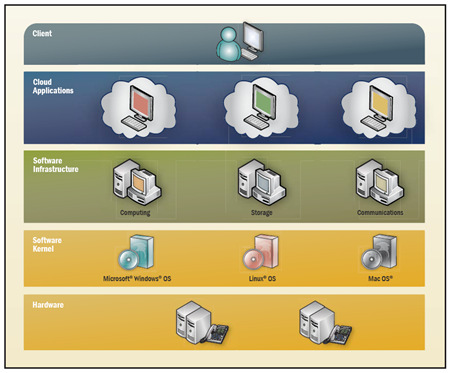
\includegraphics[scale=0.5]{img.png}
  \caption{A An architecture of the layer model of cloud computing}
  \end{center}
 \end{figure} 
 \section{Cloud Service Deployment and Consumption Models}
 Regardless of the delivery model utilized (SaaS, PaaS, IaaS) there are four primary ways in which cloud
services are deployed. Cloud integrators can play a vital role in
determining the right cloud path for a specific organization.
 \subsection{Public cloud:}Public clouds are provided by a designated service provider and may offer either a single-
tenant (dedicated) or multi-tenant (shared) operating environment with all the benefits and functionality
of elasticity and the accountability/utility model of cloud. The physical infrastructure is generally owned
by and managed by the designated service provider and located within the provider’s data centers (off-
premises). All customers share the same infrastructure pool with limited configuration, security
protections, and availability variances. One of the advantages of a public cloud is that they may be larger
than an enterprise cloud, and hence they provide the ability to scale seamlessly on demand.
 \subsection{Private cloud:}
 Private clouds are provided by an organization or their designated services and offer a
single-tenant (dedicated) operating environment with all the benefits and functionality of elasticity and
accountability/utility model of cloud. The private clouds aim to address concerns on data security and
offer greater control, which is typically lacking in a public cloud. There are two variants of private clouds:
(i) on-premise private clouds and (ii) externally hosted private clouds. The on-premise private clouds, also
known as internal clouds are hosted within one’s own data center. This model provides a more
standardized process and protection, but is limited in aspects of size and scalability. IT departments would
also need to incur the capital and operational costs for the physical resources. This is best suited for
applications which require complete control and configurability of the infrastructure and security. As the
name implies, the externally hosted private clouds are hosted externally with a cloud provider in which
the provider
 \subsection{Hybrid cloud:}
 Hybrid clouds are a combination of public and private cloud offerings that allow for
transitive information exchange and possibly application compatibility and portability across disparate
cloud service offerings and providers utilizing standard or proprietary methodologies regardless of
ownership or location. With a hybrid cloud, service providers can utilize third party cloud providers in a
full or partial manner, thereby increasing the flexibility of computing. The hybrid cloud model is capable
of providing on-demand, externally provisioned scale. The ability to augment a private cloud with the
resources of a public cloud can be used to manage any unexpected surges in workload.
 \subsection{Managed cloud:}
Managed clouds are provided by a designated service provider and may offer either a
single-tenant (dedicated) or multi-tenant (shared) operating environment with all the benefits and
functionality of elasticity and the accountability/utility model of cloud. The physical infrastructure is
owned by and/or physically located in the organizations’ data centers with an extension of management
and security control planes controlled by the designated service provider.
The notion of public, private, managed and hybrid when describing cloud services really denotes the
attribution of management and the availability of service to specific consumers of the services. Table 1
summarizes various features of the four cloud deployment models.
When assessing the impact a particular cloud service may have on one’s security posture and overall
security architecture, it is necessary to classify the assets/resource/service within the context of not only
its location but also its criticality and business impact as it relates to management and security. This
means that an appropriate level of risk assessment is performed prior to entrusting it to the vagaries of the
cloud. In addition, it is important to understand various tradeoffs between
the various cloud service models:

\begin{itemize}
\item Generally, SaaS provides a large amount of integrated features built directly into the offering with
the least amount of extensibility and in general a high level of security (or at least a responsibility
for security on the part of the service provider).
\item PaaS offers less integrated features since it is designed to enable developers to build their own
applications on top of the platform, and it is, therefore, more extensible than SaaS by nature.
However, this extensibility features trade-offs on security features and capabilities.
\item IaaS provides few, if any, application-like features, and provides for enormous extensibility but
generally less security capabilities and functionalities beyond protecting the infrastructure itself,
since it expects operating systems, applications and contents to be managed and secured by the
customers.
\end{itemize}
In summary, form security perspective, in the three service models of cloud computing, the lower
down the stack the cloud service provider stops, the more security capabilities and management the
customer is responsible for implementing and managing themselves.

\chapter{Data Security for Cloud Storage System Using Role Based Access Control}
\section{Introduction}
Sharing of resources on cloud can be done on large scale which is cost effective and location independent. Resources on the cloud can be deployed by the service providing person or company and used by the client.
It also shares necessary software’s and on-demand tools for various IT Industries. 
Cloud provides many advantages as storing information on the cloud gives almost unlimited storage capacity;
easy access to information gives access permission to data stored on cloud from anywhere if user is registered to it.
On other side, cloud got many issues regarding security especially on Data theft, Data loss and Privacy.
Protecting cloud from unauthorized users and other threats is a very important task for security providers who are in charge of the cloud as secure cloud is always reliable source of information.
A Cloud is said to be good only when it is reliable and provides better security to customers. Even if vendor is providing secure cloud, the vendor should make sure who can access the data and who maintains the server.
\section{Security issues associated with the cloud}
Cloud computing and storage solutions provide users and enterprises with various capabilities to store and process their data in third-party data centers.
Organizations use the Cloud in a variety of different service models (SaaS, PaaS, and IaaS) and deployment models (Private, Public, Hybrid, and Community).
There are a number of security concerns associated with cloud computing.
These issues fall into two broad categories: security issues faced by cloud providers (organizations providing software-, platform-, orinfrastructure-as-a-service via the cloud) and security issues faced by their customers (companies or organizations who host applications or store data on the cloud).
The responsibility is shared, however. The provider must ensure that their infrastructure is secure and that their clients’ data and applications are protected while the user must take measures to fortify their application and use strong passwords and authentication measures.
When an organization elects to store data or host applications on the public cloud, it loses its ability to have physical access to the servers hosting its information. 
As a result, potentially sensitive data is at risk from insider attacks.
According to a recent Cloud Security Alliance Report, insider attacks are the third biggest threat in cloud computing.
Therefore, Cloud Service providers must ensure that thorough background checks are conducted for employees who have physical access to the servers in the data center.
Additionally, data centers must be frequently monitored for suspicious activity.
In order to conserve resources, cut costs, and maintain efficiency, Cloud Service Providers often store more than one customer's data on the same server.
As a result, there is a chance that one user's private data can be viewed by other users (possibly even competitors).
To handle such sensitive situations, cloud service providers should ensure properdata isolation and logical storage segregation.
The extensive use of virtualization in implementing cloud infrastructure brings unique security concerns for customers or tenants of a public cloud service. Virtualization alters the relationship between the OS and underlying hardware - be it computing, storage or even networking. This introduces an additional layer - virtualization - that itself must be properly configured, managed and secured.
Specific concerns include the potential to compromise the virtualization software, or "hypervisor". While these concerns are largely theoretical, they do exist.
For example, a breach in the administrator workstation with the management software of the virtualization software can cause the whole datacenter to go down or be reconfigured to an attacker's liking.
\section{Based Access Control }
Role-based access control provides a better security solution for accessing data on cloud.
Roles in RBAC are mapped to access permissions , and all users are mapped to appropriate roles and receive access permissions only through the roles to which they are assigned, or through hierarchical roles, roles get access permission.
Within an organization, there may be number of users and types of permission, whose role and accordingly access differs. Controlling all access through roles gives benefit to organization and it also simplifies the management. 
Typically, role-based access control model has three essential structures; users permissions and roles.
A role is a higher level representation of access control.
User correspond to real world users of the computing system.
User authorization can be accomplished separately; assigning users to existing roles and assigning access privileges for objects to roles.
Permissions gives a description of the access users can have to objects in the system and roles gives a description of the functions of userswithin an organization.
In RBAC, there is hierarchical structure; a role can inherit access permission from another role.
Following diagram shows relationship between users, roles and permissions.
Relation between users, roles and permissions Data owner uses cryptographic techniques to protect data from unauthorized access for providing protection to the privacy of their data and only those users can access data who have access permission. Users need to satisfy access policies to access data.
If user satisfy the access policies, user can decrypt data by using his private key. The role based access policies are strengthened by using role-based encryption scheme (RBE).
\section{Cloud security controls}
Cloud security architecture is effective only if the correct defensive implementations are in place.
An efficient cloud security architecture should recognize the issues that will arise with security management.
The security management addresses these issues with security controls.
These controls are put in place to safeguard any weaknesses in the system and reduce the effect of an attack.
While there are many types of controls behind a cloud security architecture, they can usually be found in one of the following categories: 
\subsection{Deterrent controls} 
These controls are intended to reduce attacks on a cloud system.
Much like a warning sign on a fence or a property, deterrent controls typically reduce the threat level by informing potential attackers that there will be adverse consequences for them if they proceed.
Some consider them a subset of preventive controls.
\subsection*{Preventive controls}
Preventive controls strengthen the system against incidents, generally by reducing if not actually eliminating vulnerabilities.
Strong authentication of cloud users, for instance, makes it less likely that unauthorized users can access cloud systems, and more likely that cloud users are positively identified.
\subsection*{Detective controls}
Detective controls are intended to detect and react appropriately to any incidents that occur.
In the event of an attack, a detective control will signal the preventative or corrective controls to address the issue.System and network security monitoring, including intrusion detection and prevention arrangements, are typically employed to detect attacks on cloud systems and the supporting communications infrastructure.
\subsection*{Corrective controls} 
Corrective controls reduce the consequences of an incident, normally by limiting the damage.
They come into effect during or after an incident.
Restoring system backups in order to rebuild a compromised system is an example of a corrective control.
\section{Dimensions of cloud security}
It is generally recommended that information security controls be selected and implemented according and in proportion to the risks, typically by assessing the threats, vulnerabilities and impacts.
Cloud security concerns can be grouped in various ways;
Gartner named seven while the Cloud Security Alliance identified fourteen areas of concern.
Cloud Application Security Brokers (CASB) are used to add additional security to cloud services.
\section{Security and privacy}
\subsection{Identity management }
Every enterprise will have its own identity management system to control access to information and computing resources.
Cloud providers either integrate the customer’s identity management system into their own infrastructure, using federation or SSO technology, or a biometric-based identification system, or provide an identity management solution of their own.
CloudID, for instance, provides a privacy-preserving cloud-based and cross-enterprise biometric identification solutions for this problem.
It links the confidential information of the users to their biometrics and stores it in an encrypted fashion.
Making use of a searchable encryption technique, biometric identification is performed in encrypted domain to make sure that the cloud provider or potential attackers do not gain access to any sensitive data or even the contents of the individual queries.
\subsection*{Physical security }
Cloud service providers physically secure the IT hardware (servers, routers, cables etc.)
against unauthorized access, interference, theft, fires, floods etc.
and ensure that essential supplies (such as electricity) are sufficiently robust to minimize the possibility of disruption.
This is normally achieved by serving cloud applications from 'world-class' (i.e. professionally specified, designed, constructed, managed, monitored and maintained) data centers.
\subsection*{Personnel security}
Various information security concerns relating to the IT and other professionals associated with cloud services are typically handled through pre-, para- and post-employment activities such as security screening potential recruits, security awareness and training programs, proactive
\subsubsection*{Privacy}
Providers ensure that all critical data (credit card numbers, for example) are masked or encrypted and that only authorized users have access to data in its entirety. Moreover, digital identities and credentials must be protected as should any data that the provider collects or produces about customer activity in the cloud.
\chapter{Effective Data Access Control for Multi-Authority Cloud Storage Systems}
\begin{abstract}
Ciphertext-Policy Attribute-based Encryption (CP-ABE) is a promising
technique for access control of encrypted data, which requires a trusted authority to
manage all the attributes and distributes keys in the system. In multi-authority cloud
storage systems, the users’ attributes come from different domains each of which
is managed by a different authority. However, existing CP-ABE schemes cannot be
directly applied to data access control for multi-authority cloud storage systems, due
to the inefficiency of decryption and revocation. 
\end{abstract}

\section{Introduction}

Cloud  storage  is  an  important  service  of cloud  computing,  which  offers  services  for  data owners  to  host their  data  in  the  cloud.  This  new paradigm  of  data  hosting  and  data  access  services introduces a great challenge to data access control. Because the cloud server cannot be fully trusted by data  owners,  this  has been  solved  by  using  the attribute  based  encryption  in  the  previous  methods. \newline \newline 
[1]. In the previous method, the data owner defines the  access  policies  and  encrypts  data  according  to the  policies.  Each  user  will  be  issued  a  secret  key reflecting its attributes. A user can decrypt the data only    when    its    attributes    satisfy    the    access policies.There  are  two  types  of  CP-ABE  systems: single-authority CP-ABE [2], [3], [4], [5] where all attributes  are  managed  by  a  single  authority,  and multi-authority  CP-ABE   [6],    [7],    [8]    where attributes  are  from  different  domains and managed by different authorities. Multi-authority CP-ABE is more  appropriate  for  data  access  control  of  cloud storage systems, as users may hold attributes issued by  multiple  authorities  and  data  owners  may  also share  the  data  using  access  policy defined  over attributes from different authorities.In  multi-authority  cloud  storage  systems,  users’ attribute scan be changed dynamically. A user may be  entitled  some  new  attributes  or  revoked  some current  attributes.   And   his   permission   of   data access   should   be   changed   accordingly.  \newline \newline In   the existing  system the  attribute  changes  dynamically but  still  the  user  can  able  to  access  the  data  even after revocation. In  this  paper,  I  first  propose  a  revocable  Multi-authority system in which the data can be shared by the  user  by attribute  based  encryption,  Second  we encrypt the attribute and send the encrypted private key to the user

\section{DATA FLOW DIAGRAM:}


\begin{figure}
\centering
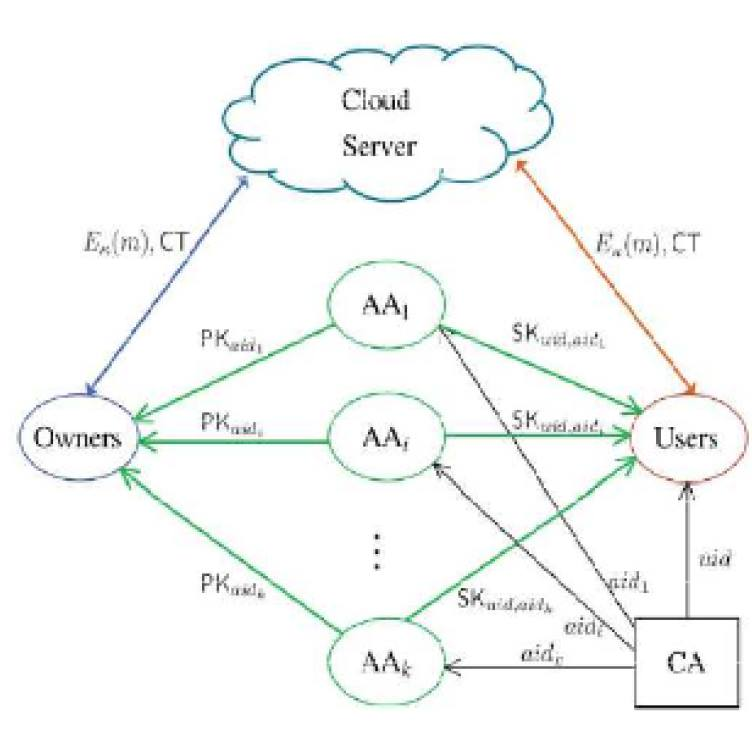
\includegraphics[width=0.8\textwidth]{ew.png}
\caption{\label{fig:SYSTEM ARCHITECTURE}}
\end{figure}


1. The DFD is also called as bubble chart. It is
a simple graphical formalism that can be
used to represent a system in terms of input
data to the system, various processing carried
out on this data, and the output data is
generated by this system. \newline \newline
2. The data flow diagram (DFD) is one of the
most important modeling tools. It is used to
model the system components. These
components are the system process, the data
used by the process, an external entity that
interacts with the system and the information
flows in the system.\newline \newline
3. DFD shows how the information moves
through the system and how it is modified by
a series of transformations. It is a graphical
technique that depicts information flow and
the transformations that are applied as data
moves from input to output.\newline \newline
4. DFD is also known as bubble chart. A DFD
may be used to represent a system at any
level of abstraction. DFD may be partitioned
into levels that represent increasing
information flow and functional detail.

\begin{figure}
\centering
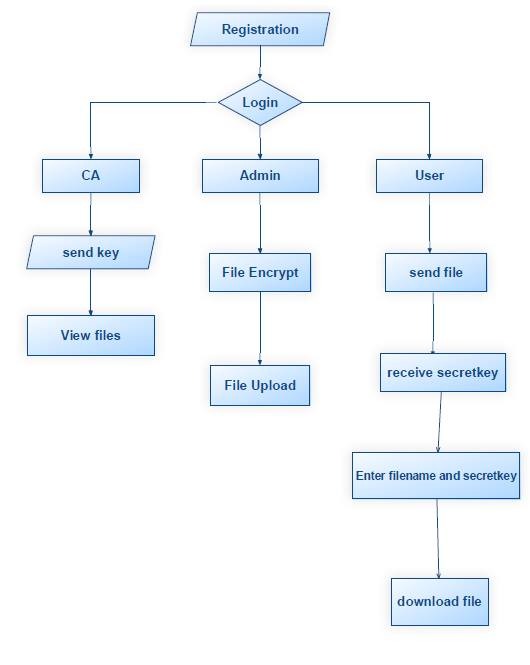
\includegraphics[width=0.8\textwidth]{dsf.png}
\caption{\label{fig:}}
\end{figure}

\section{MODULES DESCRIPTION:}
\subsection{Certificate Authority:}

The CA is a global trusted
certificate authority in the system. It sets up the
system and accepts the registration of all the users and
AAs in the system. For each legal user in the system,
the CA assigns a global unique user identity to it and
also generates a global public key for this user.
However, the CA is not involved in any attribute
management and the creation of secret keys that are
associated with attributes. For example, the CA can be
the Social Security Administration, an independent
agency of the United States government. Each user
will be issued a Social Security Number (SSN) as its
global identity.


\subsection{Attribute Authorities:}

Every AA is an independent
attribute authority that is responsible for entitling and
revoking user’s attributes according to their role or
identity in its domain. In our scheme, every attribute
is associated with a single AA, but each AA can
manage an arbitrary number of attributes. Every AA
has full control over the structure and semantics of its
attributes. Each AA is responsible for generating a
public attribute key for each attribute it manages and a
secret key for each user reflecting his/her attributes.

\subsection{Data Consumers:}

A user may be entitled a set of attributes
which may come from multiple attribute authorities.
The user will receive a secret key associated with its
attributes entitled by the corresponding attribute
authorities.

\subsection{Data Owners:}
Each owner first divides the data into
several components according to the logic
granularities and encrypts each data component with
different content keys by using symmetric encryption
techniques. Then, the owner defines the access
policies over attributes from multiple attribute
authorities and encrypts the content keys under the
policies.

\subsection{Cloud Server:}

Then, the owner sends the encrypted
data to the cloud server together with the ciphertexts.
They do not rely on the server to do data access
control. But, the access control happens inside the
cryptography. That is only when the user’s attributes
satisfy the access policy defined in the cipher text; the
user is able to decrypt the cipher text. Thus, users with
different attributes can decrypt different number of
content keys and thus obtain different granularities of
information from the same data

\section{System and Security Model}

\subsection{System Model}
In this section, we consider a secure cloud storage system for multiple authorities, as shown
in Fig.3. The system model in this paper involves five different entities: the global certificate
authorities (CAs), the attribute authorities (AAs), the cloud server (server), the data owners
(owners) and the data consumers (users).

\begin{figure}
\centering
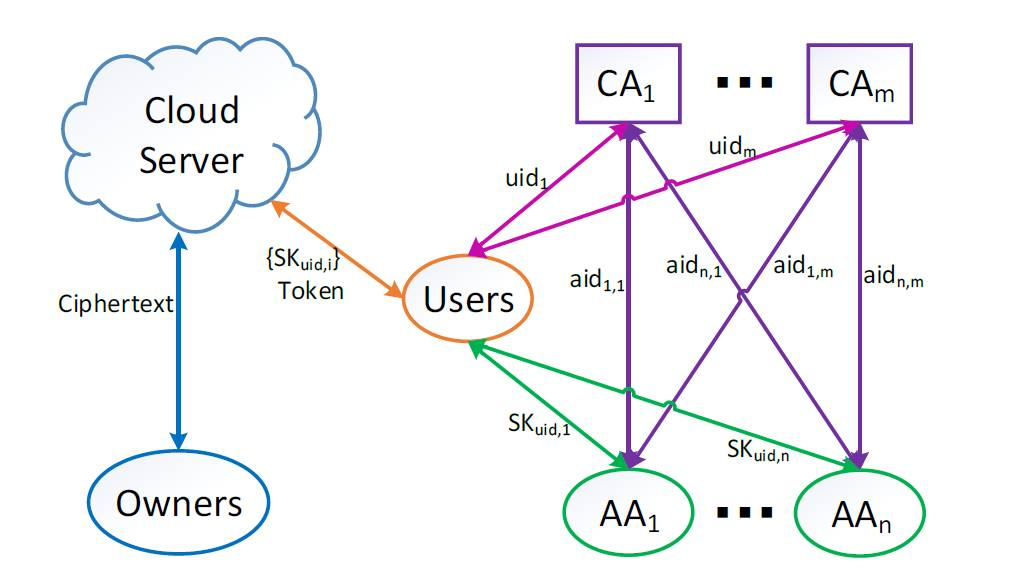
\includegraphics[width=0.8\textwidth]{fg.png}
\caption{\label{fig:3}}
\end{figure}

\subsection{Security Model}

We consider the case that the server may send the owners’ data to the users who do not
have access permission in cloud storage systems. We assume that the server will execute
correctly the task assigned by the attribute authority but the server is also curious about the
content of the encrypted data. The users who are dishonest may collude to obtain
unauthorized access to data. The AA can be corrupted or compromised by the attackers. The
CA may come across outage and security breaches in the cloud storage systems.
This section describes the security model for multi-authority CP-ABE systems by the
following game between a challenger and an adversary. Similar to the identity-based
encryption schemes [10]–[11], the security model allows the adversary to query for any secret
keys that cannot be used to decrypt the challenge ciphertext. We assume that the adversaries
can corrupt authorities only statically similar to [18], but key queries are made adaptively.




\end{document}
